
\chapter{The Basics}\label{ch:basics}


\section{Pre-conceptions}

If this were a mathematics course, then we would start by very carefully defining words like \emph{vector} and \emph{matrix}. As a physics student, you already have a working definition of these words. It is probably something like this:
%
\begin{quote}
A vector has a magnitude and a direction. We write a vector as an array of three numbers arranged in a column. A matrix is an array of nine numbers arranged in a $3\times 3$ block. There is a rule for how to apply (multiply) the matrix to the vector to produce a new vector.
\end{quote}

The problem is that you already know too much to learn linear algebra as a mathematics student. You have already seen the tip of the iceberg and so have preconceptions about what vectors are and how they work. You may remember from freshman mechanics that forces are vectors. So are momenta and velocities. You may also recall the idea of a force field---like the electric field---which is actually a whole bunch of vectors: one for each point in space. Examples of matrices are a little more subtle: you may recall that you can represent rotations as matrices. Speaking of rotations, there was another thing that showed up called the moment of inertia \emph{tensor}. It looked like a matrix, but we never called it the ``moment of inertia matrix.'' What the heck is a tensor, anyway?

And so, you see that starting this course like a mathematics course could cause trouble. The mathematics professor would start by defining a vector. That definition will say nothing about magnitudes or directions, and will not even say anything about arrays of numbers. That definition will clash with the hard-earned intuition that you built from your physics education thus far. It will be perplexing, and may make you feel rather unhappy. What do these mathematicians know, anyway? Or maybe its the physics that is wrong, or have we just completely misunderstood everything and we are just now noticing that we are hopelessly lost? We begin to spiral into a black hole of confusion.

\begin{quote}
Fortunately, \emph{this is not a mathematics course.}
\end{quote}

As a consequence, we will not give a rigorous definition of a vector. We start with a familiar definition of vectors and lay out which qualities are general, and which properties are specific. Then we will come to appreciate the approximation that ``\emph{everything is a vector}.'' So let us start with something comfortably familiar, even though it constitutes only the simplest example of a vector.


\section{Real Three-Vectors}

Let us write $\vec{v}$ to be a vector. This is a standard convention for writing a vector. In this course we will use a few different notations for vectors according to convenience. Notation is neither physics nor mathematics, it is simply a shorthand for a physical or mathematical idea. 

% At this point, you may wonder \emph{what is a vector, anyway?} Maybe a vector is a column with three numbers that represent coordinates in three-dimensional space:
In fact, let us focus on a particular type of vector: \textbf{real three vectors}\index{three vector}. These are the familiar vectors that we can write as a column of three numbers that effectively represent the coordinates in three-dimensional space:
\begin{align}
    \vec{v} = 
    \begin{pmatrix}
        x\\ y\\ z
    \end{pmatrix} \ ,
\end{align}
where $x$, $y$, and $z$ are real numbers. These numbers are called the \textbf{components} of the vector $\vec{v}$.

\begin{exercise}
There is something very perverse about this ``vector.'' The variable names $x$, $y$, and $z$ imply that $\vec{v}$ is something that physicists like to call a ``position vector.'' If you say this to a mathematician they will vomit. By the end of this course, you should appreciate why the notion of a position vector makes no sense. \emph{Hint:} You may have some intuition for this already: a velocity vector tells you about the instantaneous motion of a particle relative to its present position. Try to write the analogous statement for a ``position vector.\footnote{I am not a mathematician, but you see that even I have to write ``position vector'' in condescending quotation marks. In lecture I use even more condescending air quotes.}''
\label{ex:position:vector}
\end{exercise}

This three-dimensional space is called [three-dimensional] \textbf{real space} and we write it as $\RR ^3$. This is because a vector is an element of three-dimensional real space specified by \emph{three} real numbers. 

Three-dimensional real space is an example of a \textbf{vector space}\index{vector space}, which is just a stupidly formal way of saying that it is where vectors live. Vectors are \emph{elements} of a vector space. A vector space is the set of all possible allowed vectors of a given type. For $\RR ^3$, the vector space is composed of all possible triplets of real numbers. 


\begin{example} It should be no surprise that we can imagine real two-dimensional space, $\RR ^2$. This is a vector space where each vector may be written as two real numbers. You can also imagine writing real four-dimensional space, $\RR ^2$, or complex two dimensional space, $\mathbbm{C}^2$. 
\end{example}

From the above example, you should have some intuition for what the \textbf{dimension}\index{dimension} of a vector space means: the dimension counts how many numbers you need to specify a vector. For real vector spaces, $\RR ^d$, the dimension is the number $d$. We will always assume that $d$ is a positive integer.\sidenote{The notion of a non-integer-dimensional space does show up occasionally. These do not even have to be particularly exotic: you can look up the dimension of a fractal.}





\section{Vectors and Numbers}

% We now make some general statements about vector spaces. These apply to all vector spaces, not just $\RR ^3$, but you can keep $\RR ^3$ in mind as we go over them. 

We should be clear that there are now two different kinds of objects: \emph{vectors} and \emph{numbers}. We will have all sorts of notation for vectors, but let us write them with a boldfaced Roman letter for now, e.g.~$\vec{v}$. We typically write numbers as lowercase italicized Roman letters like $a$ or sometimes Greek letters like $\alpha$. These two types of objects are similar, except vectors do not have a built-in definition for multiplication, see Table~\ref{table:vectors:numbers}.

\begin{table}
    \renewcommand{\arraystretch}{1.3} % spacing between rows
    \centering
    \begin{tabular}{ @{} lll @{} } \toprule % @{} removes space
         & Vectors & Numbers 
        \\ \hline
        Addition (commutative, associative) & \cmark & \cmark 
        \\
        Additive null element & $\vec{0}$ & 0
        \\
        Additive inverse element & $\vec{v} + (-\vec{v}) = 0$ & $a + (-a) = 0$
        \\
        Multiplication of two of these objects & \textcolor{red}{\xmark} & \cmark 
        \\
        Multiplication by a number (distributive) & \cmark & \cmark \,(same as above)
        \\
        Collection of all allowed objects (space) & vector space & field (``numbers'') 
        \\
        Example of a space & $\RR ^3$ & $\RR $
        \\ \bottomrule
    \end{tabular}
    \caption{
        What you can do with vectors compared to numbers. The glaring difference is that we cannot multiply two vectors. We will need to invent additional mathematical structure to define vector multiplication.
        \label{table:vectors:numbers}
  }
\end{table}

You already know everything there is to know about numbers.\sidenote{Formally, what I mean by `number' is what mathematicians call a \emph{field}. This simply means some objects where one can add, subtract, multiply, and divide as you would expect. This term is a little tedious for us because physicists usually mean something else when they say `field.' Usually we mean something like the electric field or the field associated with the Higgs boson.} Most relevant is that you can multiply numbers with each other (including division, the inverse of multiplication) and you can add them together (including subtraction). For the first part of this course, we will focus on real numbers, $\RR $. Later we will also allow for complex numbers, $\mathbbm{C}$. 

Like numbers, vectors can be added and subtracted. In fact, vector arithmetic turns out to be very similar to `number arithmetic.' However, unlike numbers, there is no obvious definition for vector multiplication. This leads to the idea of \emph{defining} functions for various kinds of vector multiplication. Linear algebra is the study of a particular class of these functions. The dot product, for example, which takes two vectors and returns a number, is something we have to ``make up'' and attach to a vector space.



\section{Notation: Indices}

One theme in this course is that we will repeatedly refine our notation to suit our needs. Let us introduce an \emph{index} notation where we write the components of vectors $\vec{v}$ and $\vec{w}$ as follows:
\begin{align}
    \vec{v}
    &=
    \begin{pmatrix}
        v^1 \\ v^2 \\ v^3
    \end{pmatrix}
    &
    \vec{w}
    &=
    \begin{pmatrix}
        w^1 \\ w^2 \\ w^3
    \end{pmatrix} \ .
\end{align}
We see that a boldfaced Roman letter, $u$, corresponds to a vector. The \emph{components} of the vector are $u^1$, $u^2$, $u^3$. The ``$x$-component'' of $\vec{u}$ is called $u^1$: we use the same letter as the vector, but italicized rather than boldfaced. The upper index is \emph{not} some kind of power, it simply means ``the first component.'' 

\begin{example}
If you see $\vec{s}$, this is understood to be a vector that has multiple components. If it is a three-vector, it has three components. If you see $s^2$, then this means that this is the \emph{second component} of the vector $\vec{s}$. The component of a vector is a number. 
\end{example}

You may worry that this notation introduces ambiguity. If we see $q^2$, is this the square of some number $q$, or is it the second component of some vector $\vec{q}$? The answer depends on context. You should avoid choosing variable names where there is ever the potential for ambiguity. If you have a vector that you call $\vec{q}$, then do not use the letter $q$ for anything else.

\sidenotetext{It is a personal pet peeve of mine that some first year courses for physics majors are sloppy about this. The instructors should know that they are building the foundation for understanding quantum mechanics and special relativity: they should start developing \emph{good} mathematical habits early on. }
\begin{example}
Some courses\sidenotemark write vectors as rows: $\vec{v}=\begin{pmatrix}
    v^1 & v^2 & v^3
\end{pmatrix}$ \ . Even more annoying to me, they may write everything with a lower index, $\vec{v}=\begin{pmatrix}
    v_1 & v_2 & v_3
\end{pmatrix}$ \ . There is nothing \emph{wrong} with this, certainly in classes where there is only one type of vector. However, in order to make full use of linear algebra, we need to treat so-called column vectors separately from so-called row vectors. To do this, we introduce a new set of notation where the heights of the indices are important. Eventually we will get rid of the notion of rows versus columns altogether---but the notion of upper and lower index will remain.
\end{example}


You know from $\RR ^3$ that you can add together any two vectors $\vec{v}$ and $\vec{w}$.
% 
Let us call this sum $\vec{u}$ so that $\vec{u}\equiv \vec{v}+\vec{w}$. Then we can succinctly write the components of $\vec{u}$ in one line:
\begin{align}
    u^i = v^i + w^i \ .
    \label{eq:u:v:plus:w:index}
\end{align}
The variable $i$ is called an \textbf{index}\index{index}. What values does the index take? In this example, it is 
clear that \eqref{eq:u:v:plus:w:index} holds for $i=1,2,3$. That is, $i$ takes values from 1 to the dimension of the space. The typical convention is that we do not have to state the range of index values because it should be understood from the space itself. 

With that in mind, it should be clear that if $\vec{q}$ is the difference of two vectors, then the components of $\vec{q}$ may be succinctly written:
\begin{align}
\vec{q} &= \vec{v}-\vec{w}    
&
&\Leftrightarrow
&
q^i &= v^i - w^i \ .
\end{align}
In fact, as physicists we typically use the two statements above interchangeably. If you know the components of a vector, then you know the vector.


\section{Arithmetic and linear combinations}

All vector spaces allow addition and subtraction. This is defined component-wise. The sum of $\vec{v}$ and $\vec{w}$ is
\begin{align}
    \vec{v}+\vec{w} = 
    \begin{pmatrix}
        v^1 + w^1\\
        v^2 + w^2\\
        v^3 + w^3
    \end{pmatrix} \ .
\end{align}
What this means is that the \emph{sum} of two vectors is also a vector. That means that if $\vec{v}$ and $\vec{w}$ are vectors in $\RR ^3$, then $(\vec{v}+\vec{w})$ is a vector in $\RR ^3$. The components of the vector $(\vec{v}+\vec{w})$ are simply the sum of the components of $\vec{v}$ and $\vec{w}$. 
% 
A few formal properties that generalize to all vector spaces:
\begin{itemize}
    \item Vector addition is associative. This means that in the sum $\vec{v}+\vec{w}+\vec{u}$, it does not matter if you add $(\vec{v}+\vec{w})$ first and then add $\vec{u}$, or if you take $\vec{v}$ and then add it to $(\vec{w}+\vec{u})$. This is the kind of `obvious' property that we tend to take for granted.
    \item Vector addition is commutative. $\vec{v}+\vec{w} = \vec{w}+\vec{v}$. This is also kind of obvious. But recall that matrix multiplication is not commutative.
    \item There is a zero vector, $\vec{0}$, that does leaves any other vector unchanged under addition. $\vec{v}+\vec{0} = \vec{v}$. This should be totally obvious. The components of $\vec{0}$ are obviously all zero.
    \item There is an additive inverse (negative vectors). If $\vec{v}$ is a vector, then $-\vec{v}$ is a vector and satisfies $\vec{v}+(-\vec{v}) = \vec{0}$.
\end{itemize}
\begin{example}
The first property implies that once you have identified one vector in a vector space, $\vec{v}$, then you can immediately have an infinite number of vectors. This is because $2\vec{v} = \vec{v}+\vec{v}$ must also be a vector. Then $3\vec{v} = 2\vec{v}+\vec{v}$ must also be a vector. And so forth.
\end{example}

We get another type of operation ``for free'' with a vector space. This is called scalar multiplication or \emph{rescaling}.

% You can multiply vectors by numbers. This is called rescaling or scalar multiplication. All the usual properties of multiplication by numbers holds: associativity, commutivity, distributive law.


\section{Rescaling: multiplication by a number}

Another operation that exists in a vector space is rescaling: we multiply a vector by a number. 
Let $\alpha$ be a number. If you want to nitpick, let us restrict $\alpha$ to be a real number. If we have a vector $\vec{v}$ with components $v^i$, then $\alpha \vec{v}$ is also a vector.\sidenote{``Also a vector'' means that it is also an element of the vector space; so $(\alpha\vec{v})$ is an element of $\RR ^3$ is $\vec{v}$ is an element of $\RR ^3$. } The components of $\alpha \vec{v}$ are
\begin{align}
    (\alpha v)^i = \alpha v^i \ ,
\end{align}
by which we mean
\begin{align}
    (\alpha\vec{v})
    =
    \begin{pmatrix}
        \alpha v^1 \\
        \alpha v^2 \\
        \alpha v^3 
    \end{pmatrix} \ .
\end{align}
The parenthesis on the left-hand side is sloppy notation to mean ``the vector that is the vector $\vec{v}$ rescaled by the number  $\alpha$.'' Another way of saying this is that there is a vector $\vec{w}\equiv \alpha\vec{v}$ whose components are $w^i = \alpha v^i$.

\begin{example}
Let us do one explicit example with numbers. Suppose the vectors $\vec{v}$ and $\vec{w}$ have components
\begin{align}
    \vec{v} &=
    \begin{pmatrix}
    \phantom{+}4.2\\
    -2.6\\
    \phantom{+}7.0        
    \end{pmatrix}
    &
    \vec{w} &=
    \begin{pmatrix}
    \phantom{+}5.3\\
    \phantom{+}2.1\\
    -2.5        
    \end{pmatrix} \ .
\end{align}
I can rescale each vector by different numbers: $\alpha = 10$, $\beta = 2$. We can consider the vector that comes from adding these rescaled vectors:
\begin{align}
    \vec{u} \equiv \alpha \vec{v} + \beta \vec{w} \ .
\end{align}
The second component of $\vec{u}$ is $u^2 = -26 + 4.2 = -21.8$.
\end{example}

At this point it is useful to define some jargon. A \textbf{scalar}\index{scalar} is a number. This is in contrast to vectors (and matrices and tensors) which we can think of as arrays of numbers. In fact, every time you see the word scalar, you should just think ``number.'' Another name for `rescaling a vector by a number' is \emph{scalar multiplication}.

\section{Linear Combination and Span}
\label{sec:linear:combination:and:span}

Based on our rules for vector space arithmetic, we know that if $\vec{v}$ and $\vec{w}$ are two vectors in our vector space and if $\alpha$ and $\beta$ are any two numbers, then
\begin{align}
    \alpha\vec{v} + \beta\vec{w} 
\end{align}
is also a vector in our vector space. We call any such sum---for any values of $\alpha$ and $\beta$---a \textbf{linear combination}\index{linear combination} of the vectors $\vec{v}$ and $\vec{w}$. You can of course generalize to the linear combination of more than two vectors, say
\begin{align}
    \alpha\vec{v} + \beta\vec{w} + \gamma\vec{u} \ .
\end{align}

Given some number of vectors---$\vec{v}$ and $\vec{w}$---you can ask what are all of the possible vectors that you can form from the linear combination of those vectors? This is a vector space.\sidenote{You may want to convince yourself that this satisfies the requirements of vector space arithmetic.} We say that this vector space is \textbf{spanned} by the vectors $\vec{v}$ and $\vec{w}$. We call this vector space $\text{Span}(\vec{v},\vec{w})$. You can extend this to even more vectors, $\text{Span}(\vec{v}, \vec{w}, \vec{u},\cdots)$.

\begin{exercise}
Show that the vector space spanned by $\vec{v}$ and $\alpha\vec{v}$ is the same as the vector space spanned by $\vec{v}$.
\end{exercise}

\begin{exercise}
If $\RR ^3$ is the space of vectors with three real components, argue that the span of any four vectors is at most $\RR ^3$ but possibly a subset of $\RR ^3$. Give an example where the span of four vectors is $\RR ^2$. 
\end{exercise}


\section{Basis vectors: an illustrative example}

Let us push this idea further. It is useful to start with an example. For simplicity, let us focus on the two-dimensional plane, $\RR ^2$. A vector in $\RR ^2$ looks like this:
\begin{align}
    \vec{v} =
    \begin{pmatrix}
        v^1 \\ v^2
    \end{pmatrix} \ .
    \label{eq:v:v1:v2}
\end{align}
Any such vector may be written as the linear combination of the following two vectors:
\begin{align}
    {\bas{e}}_1 &=
    \begin{pmatrix}
        1 \\ 0
    \end{pmatrix}
    &
    {\bas{e}}_2 &=
    \begin{pmatrix}
        0 \\ 1
    \end{pmatrix} \ .
\end{align}
Indeed, it should be obvious that 
\begin{align}
    \vec{v} &= \alpha {\bas{e}}_1 + \beta {\bas{e}}_2
    & \text{with}&
    &\alpha &= v^1
    &\beta &= v^2 \ .
    \label{eq:natural:cartesian:basis}
\end{align}
In other words, these `special' vectors ${\bas{e}}_{1,2}$ satisfy:
\begin{enumerate}
    \item Any vector in $\RR ^2$ may be written as a linear combinations of ${\bas{e}}_{1,2}$. We showed this because $\vec{v}$ in the above discussion could be any vector in $\RR ^2$. Thus $\text{Span}({\bas{e}}_{1},{\bas{e}}_{1})=\RR ^2$.
    \item The coefficients in the linear combination are precisely the components of the vector $\vec{v}$. Soon we will see that this observation is actually backwards: it is the choice that ${\bas{e}}_{1}$ are special that defines the components of a vector.
\end{enumerate}

It should be obvious that any pair of vectors that ``aren't pointing in the same direction'' can span the entire space $\RR ^2$. 
\begin{exercise}
What does ``aren't pointing in the same direction'' mean in this context? Use $\vec{v}$ and $\alpha\vec{v}$ in your answer.
\end{exercise}
We could try a different pair of vectors and consider its linear combinations:
\begin{align}
    \vec{f}_1 &=
    \begin{pmatrix}
        1\\1
    \end{pmatrix}
    &
    \vec{f}_2 &=
    \begin{pmatrix}
        0\\1
    \end{pmatrix} \ .
\end{align}
Then the vector $\vec{v}$ may be written as $\vec{v} = \alpha \vec{f}_1+ \beta\vec{f}_2$. To find $\alpha$ and $\beta$, we can simply plug in the components of $\vec{v}$ and $\vec{f}_{1,2}$ so that:
\begin{align}
    v^1 &= \alpha -\beta
    &
    v^2 &= \alpha \ .
\end{align}
In other words,
\begin{align}
    \vec{v} = (v^2) \vec{f}_1 + (v^2 - v^1)\vec{f}_2 \ .
\end{align}
These coefficients $\alpha = v^2$ and $\beta = v^2 - v^1$ may be written  in shorthand. Let's suggestively write
\begin{align}
    \vec{v} = 
    \begin{pmatrix}
        v^2\\
        v^2 - v^1
    \end{pmatrix}_{\vec{f}} \ ,
\end{align}
where we use the subscript $\vec{f}$ to mean ``coefficients with respect to $\vec{f}_{1,2}$. This looks just like a two-component vector, doesn't it?

\begin{exercise}
Let $\vec{v} \in \RR ^2$ be the following vector in two-dimensional real space:
\begin{align}
    \vec{v}=
    \begin{pmatrix}
        3\\2
    \end{pmatrix} \ .
\end{align}
Here are two vectors that span $\RR ^2$:
\begin{align}
    \vec{g}_1 &=
    \begin{pmatrix}
        2\\1
    \end{pmatrix}
    &
    \vec{g}_2 &=
    \begin{pmatrix}
        -1\\ \pp 0
    \end{pmatrix} \ .
\end{align}
What are the coefficients $\alpha$ and $\beta$ so that $\vec{v} = \alpha \vec{g}_1 + \beta \vec{g}_2$?  \emph{Answer}: $\alpha = 2$ and $\beta = 1$. 
\end{exercise}


What we're getting at is the following.  Define a set of vectors that span a space. We will call this set of vectors a \textbf{basis}\index{basis} of that space---we'll give a slightly more formal definition below. Any vector in the space can be written as a linear combination of basis vectors. For example, if $\vec{b}_{1,2}$ are a basis of $\RR ^2$, then for any vector $\vec{v}\in\RR ^2$ we may write
\begin{align}
    \vec{v} = \alpha \vec{b}_{1} + \beta \vec{b}_2 \ .
\end{align}
Then we have encoded all of the data of vector $\vec{v}$ into the coefficients $(\alpha, \beta)$. In fact, let me be more economical with my symbols and change notation a bit and write $(\alpha^1, \alpha^2) \equiv (\alpha,\beta)$ so that
\begin{align}
    \vec{v} = \alpha^1 \vec{b}_{1} + \alpha^2 \vec{b}_2 \ .
    \label{eq:R2:vec:v:in:b:components:lincomb}
\end{align}
Then I can write the information encoded in $\vec{v}$ as a column, which I will write with a subscript $b$ to distinguish it from the ``actual'' vector components, \eqref{eq:v:v1:v2}:\sidenote{We will soon see that the there is nothing holy about \eqref{eq:v:v1:v2}.}
\begin{align}
    \vec{v} = 
    \begin{pmatrix}
        \alpha^1\\
        \alpha^2
    \end{pmatrix}_{\vec{b}} \ .
    \label{eq:R2:vec:v:in:b:components}
\end{align}
The last two equations mean exactly the same thing. Now here's something cute: we can treat the two-component array\sidenote{I'm trying not to call it a vector.} on the right-hand side of \eqref{eq:R2:vec:v:in:b:components} as if it were a vector. We can do vector arithmetic on it. If we have two vectors with ``$\vec{b}$ basis components''
\begin{align}
    \vec{v}&=
    \begin{pmatrix}
        \alpha^1\\
        \alpha^2
    \end{pmatrix}_{\vec{b}} 
    &
    \vec{w}&=
    \begin{pmatrix}
        \beta^1\\
        \beta^2
    \end{pmatrix}_{\vec{b}}  \ ,
\end{align}
Then we could take linear combinations of the two with respect to two numbers $a$ and $b$:
\begin{align}
    a\vec{v} + b\vec{w} =
    (\alpha^1+\beta^1) \vec{b}_{1} + (\alpha^2+\beta^2) \vec{b}_2
    =
    \begin{pmatrix}
        \alpha^1 + \beta^1 \\
        \alpha^2 + \beta^2
    \end{pmatrix}_{\vec{b}} \ .
    \label{eq:linear:combination:in:b:basis}
\end{align}

If $\vec{v}$ and $\vec{w}$ span $\RR ^2$, then any vector in the vector space may be written as a linear combination of the form \eqref{eq:linear:combination:in:b:basis}. This means we may use the ``$\vec{b}$ basis components'' as equivalent ways of encoding a vector as the natural description \eqref{eq:v:v1:v2}. But wait a moment: what is so ``natural'' about \eqref{eq:v:v1:v2}? 

If we reverse the argument for the $\vec{b}$ basis, then we see that the ``natural'' components of the vector $\vec{v}$ in \eqref{eq:v:v1:v2} are simply the coefficients of the linear combinations of the basis vectors ${\bas{e}}_{1,2}$ in \eqref{eq:natural:cartesian:basis}. What made the basi vectors ${\bas{e}}_{1,2}$ so special, anyway? Nothing at all. 

What we've come to is that we the \emph{components} of a vector depend on the basis that we choose. In $\mathbb{R}^3$ we usually use the basis ${\bas{e}}_{1,2,3}$ where the vectors point respectively along the $\hat{x}$, $\hat{y}$, and $\hat{z}$ directions. It is kind of an ``obvious'' basis, though it completely depends on the $\hat{x}$, $\hat{y}$, and $\hat{z}$ directions having some intrinsic meaning. They often do not: we could set up our coordinate system however we wanted. In fact, \emph{nowhere} in our definition of a vector space did we even assume that a coordinate system exists!

Indeed, it's the other way around: a choice of basis vectors \emph{defines} a `coordinate system' rather than the other way around.\sidenote{Though it really is dangerous to think about a vector space as having coordinates. We will see why when we talk about vector bundles and manifolds.} All of this begs for a re-definition.





\section{Basis vectors, formally}

A \textbf{basis} is a \emph{minimal set} of vectors that span a space. Here `minimal' means that if you remove any vector from the basis, then there are vectors in the space that cannot be written as a linear combination of the remaining vectors.

\begin{example}\label{eg:over:specified:basis}
Consider the following three vectors:
\begin{align}
    \vec{v} &=
    \begin{pmatrix}
        1\\0\\0
    \end{pmatrix}
    &
    \vec{w} &=
    \begin{pmatrix}
        0\\1\\0
    \end{pmatrix}
    &
    \vec{u} &=
    \begin{pmatrix}
        1\\-1\\0
    \end{pmatrix} \ .
    \label{eq:tvu:example:basis}
\end{align}
These three vectors are \emph{not} a basis for a subspace because there are vectors that are linear combinations of $\vec{v}$, $\vec{w}$, and $\vec{u}$ that can be equivalently written as a linear combination of just $\vec{v}$ and $\vec{u}$, for example.
% 
To see this, consider the vector
\begin{align}
    \vec{t} = 4\vec{v} + 2\vec{w} + 3\vec{u} 
    =
    \begin{pmatrix}
        \pp 7 \\ -1 \\ \pp 0
    \end{pmatrix} \ .
\end{align}
This may equivalently be written as
\begin{align}
    \vec{t} = 7\vec{v} - \vec{w} \ .
\end{align}
Indeed, there are an infinite number of ways to write $\vec{t}$. Because $\vec{v} - \vec{w} + \vec{u} = 0$, you can add any multiple of this linear combination to $\vec{t}$ to leave $\vec{t}$ unchanged.
\end{example}

The \textbf{dimension} of a vector space is the number of vectors in the basis. In the example above, the vector space spanned by linear combinations of $\vec{v}$, $\vec{w}$, and $\vec{u}$ has dimension two. This is because you only need two vectors write any vector in the space as a linear combination. If you drew all of the vectors in this subspace as arrows with their base at the origin, then the arrow heads with all live on the $xy$-plane.

Here are some \emph{obvious} statements\sidenote{This means: if they are not immediately apparent, stop and think about it to make sure you understand.}:
\begin{enumerate}
    \item The zero vector cannot be part of any basis.
    \item The dimension of a vector space does not depend on the choice of basis.
    \item If you have a proposed set of basis vectors but there is a \emph{non-trivial} linear combination of those vectors that sums to zero, then the set of vectors is not a basis. Here non-trivial means ``the coefficients are not all equal to zero.'' This should be evident from Example~\ref{eg:over:specified:basis}.
    \item If any two vectors in a proposed basis are proportional to one another, then this set of vectors is not a basis.
    \item The number of components $v^i$ to describe a vector is the dimension of the vector space.
    \item In the expansion of a vector as a linear combination of basis vectors, the coefficients are unique to the vector. That is: if $\vec{v} = \sum_i \alpha^i\vec{b}_i$ for a basis $\vec{b}_{1,2,3}$, then the set of numbers $(\alpha^1, \alpha^2, \alpha^3)$ uniquely defines $\vec{v}$. There is no other combination of coefficients in a linear combination that sum to $\vec{v}$. 
    \item When describing a vector, the \emph{coefficients} of the linear combination of basis vectors and the \emph{components} of a column vector with respect to that basis are identical. This is by definition. 
\end{enumerate}
The last point is poignant. You may have believed that a vector \emph{is} the column of numbers. We want to move away from this so that we may generalize our definition. A vector is a linear combination of basis vectors, where we are remaining agnostic about what the basis vectors are. Let me say this again: \emph{the column of numbers is not the vector, it is simply a representation of a linear combination of basis vectors. All the ``vector-ness'' is encoded in the basis vectors.}\sidenote{For a sneak peek of this, you may want to jump to Section~\ref{sec:sub:abstraction:basis}.}




What is less obvious is that at this point there is \emph{no preferred basis}. Any minimal set of vectors that span a vector space is a perfectly good vector. Suppose $\vec{b}_{1,2,3}$ is one such set for $\RR ^3$. We can write the vector with respect to the coefficients of the linear combination of  $\vec{b}_{1,2,3}$ basis vectors that reproduces it. If we had another basis, $\vec{b}'_{1,2,3}$, we could write the same vector with respect to a different linear combination of the $\vec{b}'_{1,2,3}$ basis. The components of these linear combinations, say $\alpha^i$ and $\alpha'^i$, will be different because the basis elements are different. However, they represent the same vector.

In your heart, you should feel anxious. You \emph{like} the ``obvious'' basis 
\begin{align}
    {\bas{e}}_1 &=
    \begin{pmatrix}
        1 \\ 0 \\ 0
    \end{pmatrix}
    &
    {\bas{e}}_2 &=
    \begin{pmatrix}
        0 \\ 1 \\ 0
    \end{pmatrix}
    &
    {\bas{e}}_2 &=
    \begin{pmatrix}
        0 \\ 0 \\ 1
    \end{pmatrix} \ .
\end{align}
We can even call this the Cartesian basis.
It seems so natural, we even gave these basis vectors little hats to remind us how much we like them! Stop and think about what you like about this basis. I guarantee you that all of those nice features invoke mathematical machinery that are \emph{not} included in a vector space. You may like that the Cartesian basis is orthogonal and each basis vector has unit length. To this I reply: \emph{how do you measure angle or length? These are not concepts that our vector space is equipped with.} You are, of course, correct that there \emph{is} a way to \emph{define} angle and length---but that is something additional that we have to impose on the space. We will get to this shortly.


\begin{example}\label{eg:polynomial:space}
Another surprising example of a vector space is the space of polynomials of finite degree. This means functions of the form
\begin{align}
    f(x) &= a^0 + a^1 x + a^2x^2 + \cdots a^N x^N \ .
\end{align}
Finite degree means that $N$ is some integer that is not infinity.\footnote{This may seem like a silly point, but one of the key `aha' ideas in this course will be that we can do linear algebra on the space of general functions where we allow $N\to \infty$.}
To be clear, our notation has become a bit ambiguous: here $x$ is a variable and $x^n$ means $x$ to the $n^\text{th}$ power. The coefficients $a^i$, on the other hand, are numbers and $i$ is an index. We can pick the following basis:
\begin{align}
    {\bas{e}}_0 &= x^0 = 1 &
    {\bas{e}}_1 &= x^1 = x &
    {\bas{e}}_2 &= x^2 &
    \cdots&&
    {\bas{e}}_N &= x^N &
\end{align}
These `basis vectors' are actually functions that are simple monomial powers of $x$. It should be obvious (there's that phrase again) that linear combinations of these basis vectors/functions can give any function $f(x)$ of degree up to $N$. It should also be obvious that the dimension of this space is $(N+1)$; don't forget to count the ${\bas{e}}_0$ vector.\par

For example, consider the polynomial $f(x) = 3+x^2$. The linear combination of basis vectors that gives this has $a^0 = 3$, $a^2 = 1$, and all other coefficients zero:
\begin{align}
    f(x) = 3{\bas{e}}_0 + {\bas{e}}_2 \ .
\end{align}
We could represent this vector/function as a column:
\begin{align}
    f(x) = \vec{f} = 
    \begin{pmatrix}
        3 \\
        0 \\
        1 \\
        0 \\
        \vdots  \\
        0
    \end{pmatrix}
\end{align}
where $\vec{f}$ is an $(N+1)$-component column of the numbers $a^i$.
\end{example}

\begin{exercise}
Consider a vector/function $\vec{f}$ with components $f^i$ in the polynomial space in Example~\ref{eg:polynomial:space}. Now consider the vector/function $\vec{f}' \equiv df/dx$. Write out an expression for the $i^\text{th}$ component of $\vec{f}'$. \emph{Hint}: for example, the $i=1$ component is $2f^2$.
\end{exercise}



\section{The meaning of column vectors}

The previous subsection on bases\footnote{The plural of `basis' is `bases,' pronounced \emph{bay-sees}, just like the plural of `axis' is `axes' pronounced \emph{axe-sees}.} is so important that we should really emphasize the mathematical edifice that we have reverse-engineered\footnote{Do you appreciate why I say `reverse engineered' here? In mathematics classes, one woud start with some postulates for what an abstract vector is and then your usual 3-component column vectors pop out as one silly example. We have started those 3-component column vectors and used their properties to motivate a general definition of what vectors are.}
\begin{enumerate}
    \item A vector is technically \emph{not} the column of numbers that we usually say it is. That column of numbers is simply a way of writing the \emph{components} of a vector.
    \item The components of a vector are simply the coefficients of the basis vectors in the linear combination of basis vectors that sum to the vector. That is: $v^i$ is defined by $\vec{v} = v^i {\bas{e}}_i$ where the ${\bas{e}}_i$ are a set of basis vectors that we all agree upon.
    \item I never had to say what the basis vectors \emph{are}. They can be anything where linear combinations of those things are still the same type of thing. In this way, we can treat the basis vectors abstractly.
\end{enumerate}
You may be used to vectors being forces, momenta, velocities, electric fields, and so forth. We want to be able to use the same machinery of linear algebra on more general objects: particles with quantum spin, functions, the perception of colors by the human eye, and so forth.


\begin{exercise}
What happens when we do not agree on a basis? Suppose you set up a basis. Stand up. Suppose you are facing north. Your feet are at the origin. If you spread your arms out, your right hand points in the direction of your first basis element ($x$-axis, pointing east), ${\bas{e}}_1$. Your nose points in the direction of your second basis element ($y$-axis, north), ${\bas{e}}_2$. Your head points in the direction of your third basis element ($z$-axis, skyward), ${\bas{e}}_3$.

However, your friend Riley approaches you from the northeast so Riley is facing southwest. Riley decides to set up their own basis, analogous to you. Their first basis element ${\bas{r}}_1$ points in the northwest direction, their second basis element ${\bas{e}}_2$ points in the southwest direction, and their third basis element ${\bas{e}}_3$ also points skyward. 

For simplicity, assume that the length of your basis vectors are all the same---even though we haven't defined what length means. Suppose you `measure' a vector with components $v^1 = 2$, $v^2=-1$, and $v^3=1.5$. This is a vector pointing southeast and upward. What components does Riley measure with respect to their basis?
\end{exercise}



In some physics classes there is an agreed upon notion that the basis vectors are 
\begin{align}
    \bas{e}_1 &= \hat x_1 = \hat i
    &
    \bas{e}_2 &= \hat y_1 = \hat j
    &
    \bas{e}_3 &= \hat z_1 = \hat k \ .
\end{align}
This is not one of those classes. Often this \emph{canonical} basis is the obvious one to use, and we will try to use it. However, in this class you must be able to accept that we want to \emph{abstract} away the identity of the basis vectors. The basis vectors simply carry the vector-ness of a vector so that we can focus only on dealing with the \emph{components}, which we write as columns of numbers.




\section{Operations that are not (yet?) allowed}

In these definitions, we make a big deal about how the sum of two vectors \emph{is also a vector}. Or how the rescaling of a vector by a number \emph{is also a vector}. This is in contrast to operations that are either not allowed or that do not produce vectors. An example of an operation that is not allowed is adding together vectors from two different vector spaces. The following proposed sum of a vector in $\RR ^3$ with  a vector in $\RR ^2$ does not make sense:
\begin{align}
    \begin{pmatrix}
        v^1\\ v^2 \\v^3
    \end{pmatrix}
    +
    \begin{pmatrix}
        w^1\\ w^2 
    \end{pmatrix}
    =
    \; ?
\end{align}
If you find yourself adding vectors from two different vector spaces, then you have made a mistake.

Another operation that requires care is rescaling a real vector by a complex number. If $\vec{v}$ is a vector in $\RR ^3$ and we try to multiply it by a complex number, $\alpha = 2+3i$, then the resulting ``vector'' is \emph{not} a vector in $\RR^3$:
\begin{align}
    (\alpha\vec{v})^i = (2+3i)v^i \notin \RR  \ ,
\end{align}
that is: the components of $\alpha\vec{v}$ are not real numbers, and so this cannot be an element of aa vector space that is \emph{defined} to have real components. Later on we will generalize to the case of \emph{complex vector spaces}, but we will treat that with some care.\sidenote{If you want to be fancy, you can replace `number' with the mathematical notion of a \emph{field}\index{field}. Both the real numbers and the complex numbers are examples of fields. In my mind a field is just a class of number, though mathematicians have fancier definitions.}

Thus far, we have introduced the \emph{nouns} of this course: vectors. We have identified a few \emph{verbs} that let us do things with these vectors:
\begin{enumerate}
    \item Addition takes two vectors in a vector space and returns a vector in the same vector space. 
    \item Rescaling takes a vector and a number and returns a vector in the same vector space.
\end{enumerate}
We can rewrite this in the language of \emph{mappings} (or \emph{functions}) as follows. Let $V$ be a vector space, say $V=\RR ^3$. Let us write $\RR $ mean [real] numbers. Then the above statements tell us that addition and rescaling can be thought of as maps:
\begin{enumerate}
    \item Vector addition: $V\times V \to V$
    \item Rescaling: $V\times \RR  \to V$ \ .
\end{enumerate}
Do not be intimidated by the $\times$ symbol here. This ``mapping'' notation means nothing more and nothing less than the statements above.

We now know everything there is to know about the vector space $\RR ^3$. We want to learn more about functions (maps) that involve this vector space. How can we combine vectors and numbers to produce other vectors and numbers? What about more complicated objects like matrices and tensors? 

\section{Euclidean three-space}

You may object: \emph{wait! I know there are more things you can do with three-vectors!} You remember that there are two types of vector multiplication that we use in physics. The \textbf{dot product} and the \textbf{cross product}. 

In $\RR ^3$, the \textbf{dot product} is a map $V\times V \to \RR $. That means it takes two vectors and returns a number. The particular number that it returns is typically \emph{defined} to be
\begin{align}
    \vec{v} \cdot \vec{w} 
    = \sum_i v^i w^i  
    = v^1w^1 + v^2 w^2 + v^3w^3 \ .
    \label{eq:euclidean:3d:metric:intro}
\end{align}
The dot product generalizes in linear algebra. It is often called an \textbf{inner product} or a \textbf{metric} and has a few different notations that we will meet. What is important is that this dot/inner product is an \emph{additional} mathematical function that we attach to a vector space. 

Three-dimensional real space combined with the dot product/inner product/metric \eqref{eq:euclidean:3d:metric:intro} is called Euclidean three-space. In general, a vector space combined with a `dot product' is called a \textbf{metric space}. The word metric should invoke some etymological notion of measurement of distance. Indeed, the dot product is a tool that tells us how `close' two vectors are to one another---though it is not yet obvious how.

\begin{example}
Let $\mathbf{r}=(x,y,z)$ be a ``position vector'' of a point relative to the origin.\footnote{It is dangerous to use the phrase ``position vector,'' see Exercise~\ref{ex:position:vector}.} Then the distance of the point from the origin is
\begin{align}
    d = \sqrt{\vec{r}\cdot\vec{r}} =
    \sqrt{x^2+y^2 +z^2} \ .
    \label{eq:distance:in:space}
\end{align}
This gives a notion of how the dot product is related to measuring distances, but it turns out to be a bit of a red herring! The real sense in which the dot product measures the `closeness' of two vectors is the sense in which it defines an angle between those vectors. (See below.)
\end{example}


The \textbf{cross product} is a different story. You may remember the cross product from such hits as\footnote{\url{https://tvtropes.org/pmwiki/pmwiki.php/Main/YouMightRememberMeFrom}} angular momentum, $\vec{r}\times\vec{p}$. It looks like a map that takes two vectors and spits out another vector, $V\times V \to V$. Indeed, this is the case in Euclidean three-space. However, it had some funny properties compared to the dot product. For example, there was something weird with the order of the two vectors: $\vec{a}\times \vec{b}  = - \vec{b}\times \vec{a}$. It is also a bit funny that the direction of the output vector is completely different\sidenote{The technical meaning of `completely different' is \emph{orthogonal}, which we define below with the help of the metric.} from the directions of the input vectors. It will turn out that this product does not generalize as simply as the dot product, though there is a generalization called the \textbf{wedge product} which is outside the scope of this course.\sidenote{That is not to say that the wedge product is not relevant in phsyics. The wedge product features prominently in a mathematical field called \emph{differential geometry}, which is in turn the framework for general relativity. The wedge product is related to defining volumes and integration measures. You may also be interested in a field called \emph{geometric algebra} which is a related approach to the wedge product.\footnotemark}\footnotetext{e.g.\ see \url{https://www.youtube.com/watch?v=60z_hpEAtD8}}

\begin{exercise}
Define the generalization of the Euclidean three-space metric to Euclidean space in $d$ dimensions. (Easy.)
\end{exercise}

\begin{exercise}
Try to define a generalization of the cross product in two-dimensional Euclidean space. Reflect on why this is much less natural than the generalization of the dot product. 
\end{exercise}



\section{Length in Euclidean three-space}
\label{sec:Euclidean:three:length}

Euclidean three-space is real space combined with the Euclidean dot product, \eqref{eq:euclidean:3d:metric:intro}. The [Euclidean] \textbf{magnitude} (length) of a three vector $\vec{v}$ as $|\vec{v}|$ in Euclidean three-space. The magnitude is defined to be
\begin{align}
    |\vec{v}| = \sqrt{\vec{v}\cdot\vec{v}} \ .
\end{align}
This definition generalizes to Euclidean $d$-dimensional space with the appropriate generalization of the dot product.

\begin{example}
Consider the vector
\begin{align}
    \vec{v} = 
    \begin{pmatrix}
    \phantom{+}3\\-4\\\phantom{+}0    
    \end{pmatrix}
\end{align}
in Euclidean three-space. The magnitude of $\vec{v}$ is $|\vec{v}| = 5$.
\end{example}


Some references prefer to use the double bar notation, $||\vec{v}||$ for the length of a vector. This is to distinguish it from the absolute value of a number, $|-3| = 3$. We will be even more perverse: sometimes we will write $v$ to mean the magnitude of $\vec{v}$ when there is no ambiguity.

\begin{example}
Consider the vector
\begin{align}
    \vec{v} = 
    \begin{pmatrix}
    -1\\ \phantom{+}3\\ \phantom{+}2
    \end{pmatrix} \ .
\end{align}
Then the \emph{magnitude} of $\vec{v}$ is $|\vec{v}|=\sqrt{14}$. We could also write this as $v = \sqrt{14}$, but we should be careful when we write things like $v^2$ which could either mean the second component of $\vec{v}$---which is $3$---or the square of the magnitude---which is 14. 
\end{example}


We see that the dot product (metric) allows us to define length. Because the length of a vector is a number, we can divide the vector $\vec{v}$ by its its length $|\vec{v}|$ to obtain a \textbf{unit vector}:
\begin{align}
    {\bas{v}} = \frac{1}{|\vec{v}|}\vec{v} \ .
    \label{eq:eg:v:340}
\end{align}
The right-hand side is simply scalar multiplication by $|\vec{v}|\inv$. Unit vectors are useful for identifying directions.

\begin{example}
In grade school one may have learned that a vector is an arrow that has a magnitude and a direction. Unit vectors encode the `direction' of a vector.
\end{example}

\begin{example}
Let $\vec{v}$ be defined as in \eqref{eq:eg:v:340}. The unit vector associated with $\vec{v}$ is
\begin{align}
    \hat{v} = 
    \begin{pmatrix}
        \phantom{+}3/5 \\
        -4/5\\
        0
    \end{pmatrix} \ .
\end{align}

\end{example}

\section{Angle in Euclidean three-space}
\label{sec:Euclidena:three:angle}

Once you have an inner product you can define the angle, $\theta$, between two vectors, $\vec{v}$ and $\vec{w}$. This is defined as follows:
\begin{align}
    \vec{v}\cdot\vec{w} \defeq |\vec{v}||\vec{w}| \cos\theta  \ .
    \label{eq:angle:between:3:vectors}
\end{align}
\begin{exercise}
Show that the angle between two vectors only depends on their orientation and not their magnitude. 
\end{exercise}


\section{Matrix Multiplication}
\label{sec:matrix:multiplication}

A matrix is an object that acts on vectors to give you other vectors. In this way, we say that it encodes a \emph{transformation} of a vector. For simplicity, let us write this out for two-component vectors. Matrices are then $2\times2$ arrays that look like this:
\begin{align}
    M = \begin{pmatrix}
        a & b\\
        c & d
    \end{pmatrix} \ .
\end{align}
The numbers $a$, $b$, $c$, and $d$ are the components of the matrix. These act on a vector, which we shall take to be
\begin{align}
    \vec{v} = \begin{pmatrix}
        x \\ y
    \end{pmatrix} \ .
\end{align}
% 
When we multiply $\vec{v}$ by the matrix $M$ we get a new \emph{vector} which we write $M\vec{v}$. 
There is a silly rule to tell us what the components of the $M\vec{v}$ vector are.
The rule is visualized in Figure~\ref{fig:matrix:mult:2220}.
% \begin{figure}[ht]
%     % \centering
%     \sidecaption[][-2\baselineskip]{%
%         Matrix multiplication rule visualized. 
%         %
%         %% \label command inside the \sidecaption command
%         \label{fig:matrix:mult:2220}
%     }
%     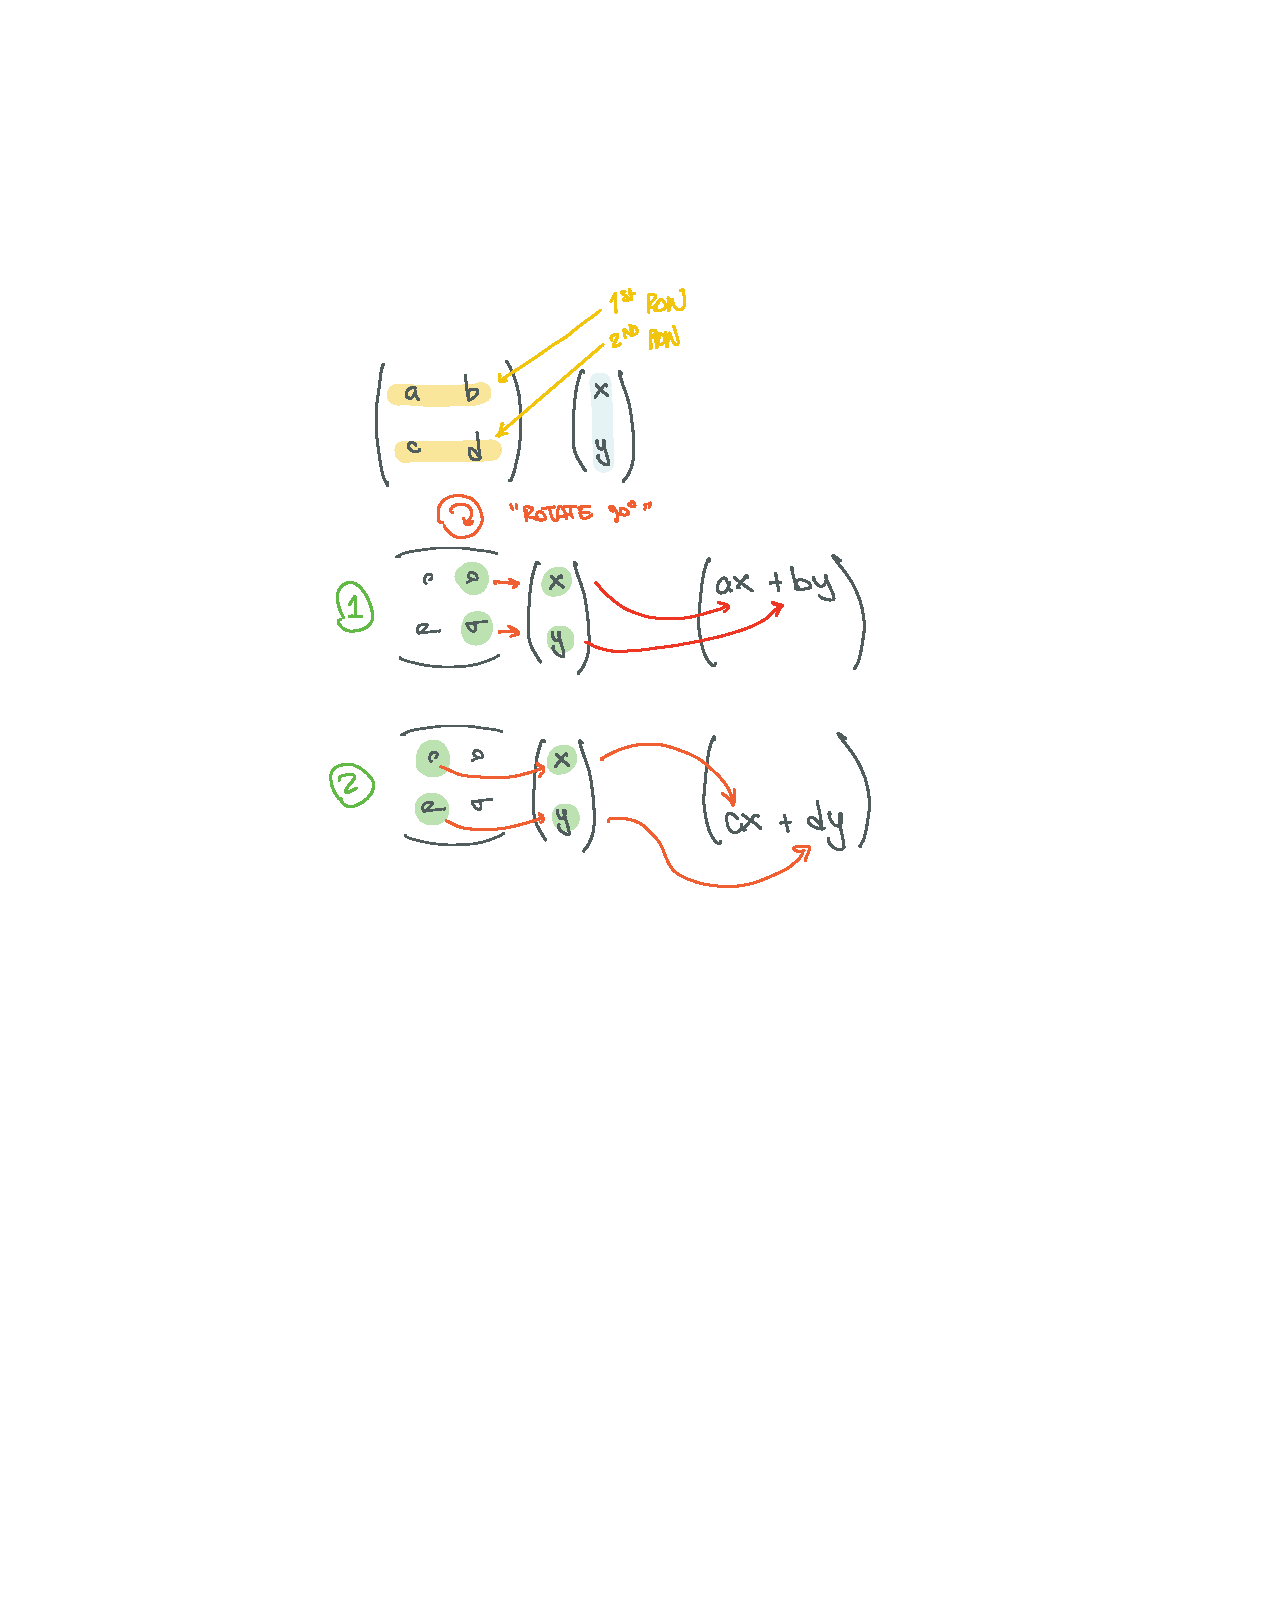
\includegraphics[width=.5\textwidth]{figures/MatrixMult_2220.pdf}
% \end{figure}
\begin{marginfigure}%[th]
    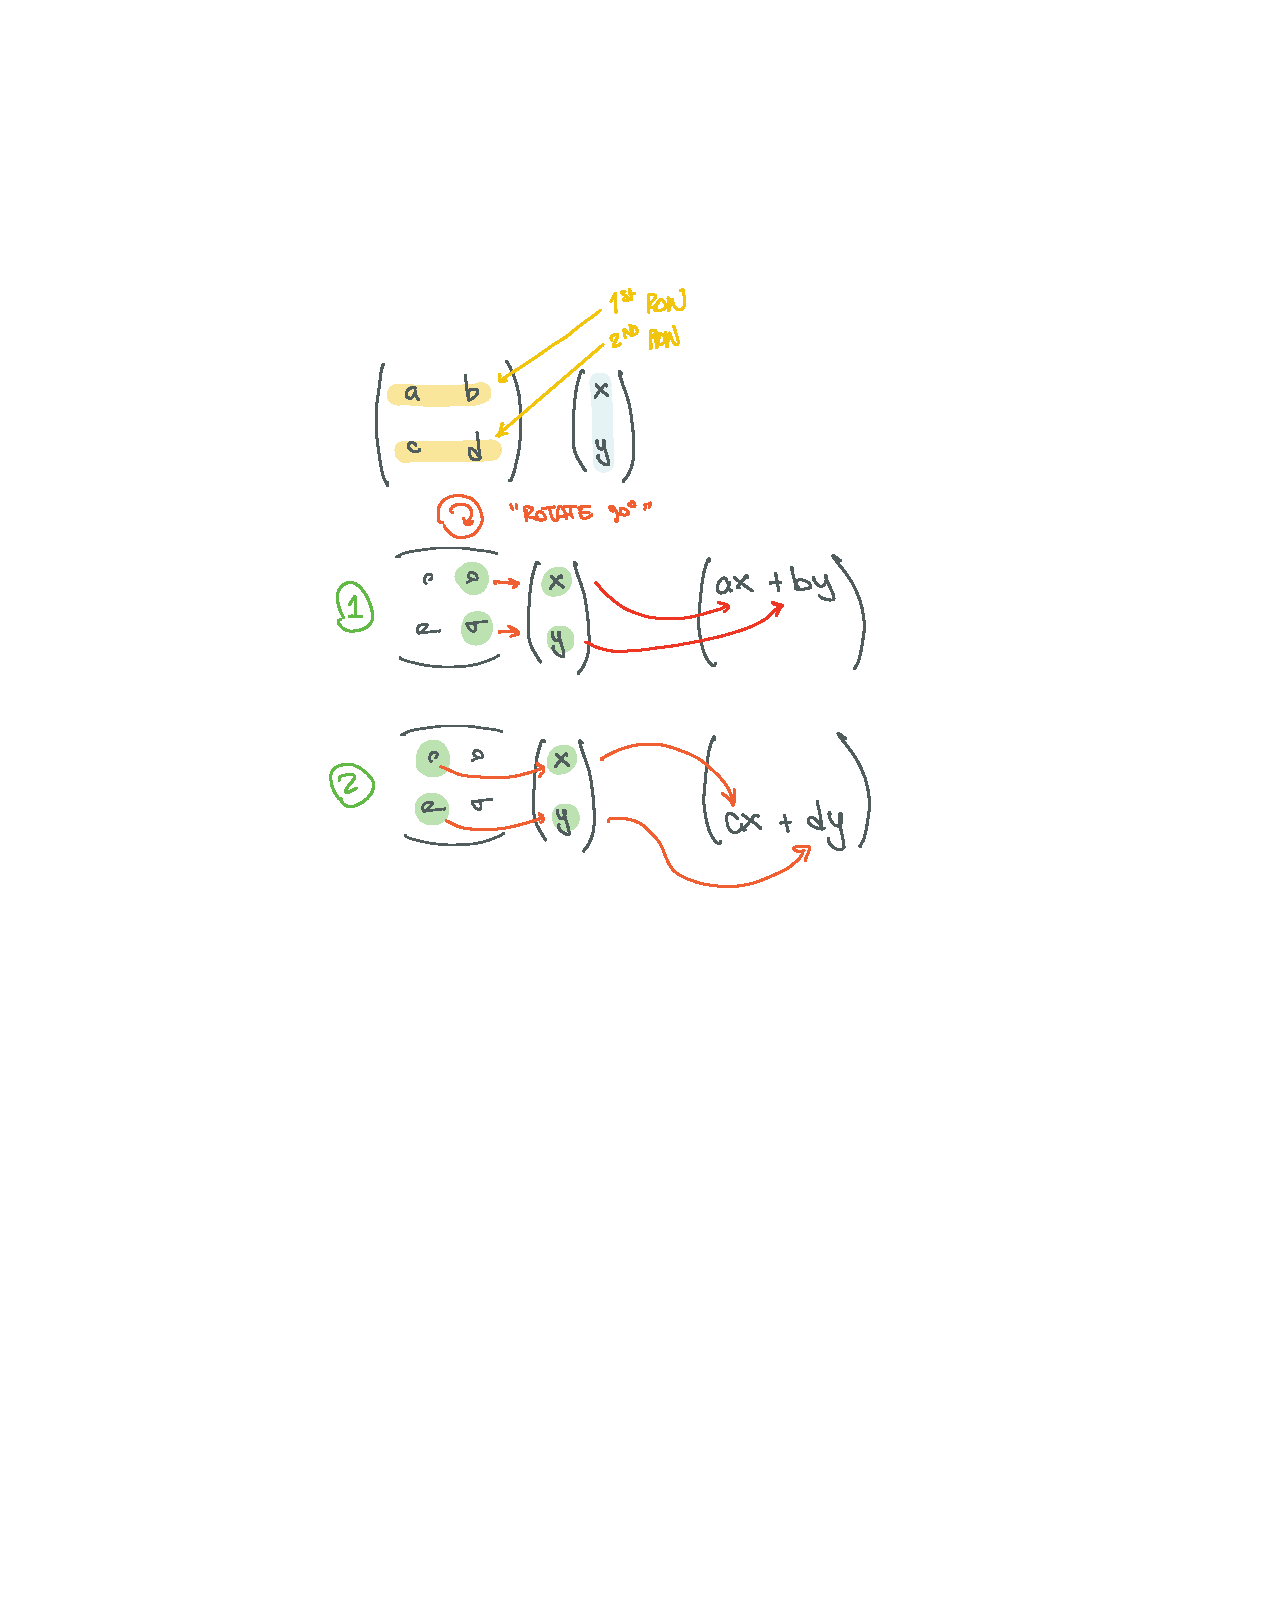
\includegraphics[width=\textwidth]{figures/MatrixMult_2220.pdf}
    \captionsetup{font={scriptsize,sf}}
    \caption{Multiplying a vector by a matrix.}
    \label{fig:matrix:mult:2220}
\end{marginfigure}
It is clunky to say the rule in words, but it goes something like this: 
\begin{enumerate}
    \item The components in the \emph{first} row of the matrix combine with the components of the column of the vector to give the \emph{first} component of $M\vec{v}$. To enact this visually,  highlight the \emph{first} row and rotate the array of numbers in $M$ clockwise by 90 degrees. The components of $M$-tipped over that are the same height as the corresponding components of $\vec{v}$ are multiplied and each product is summed together. This sum is the \emph{first} component of $M\vec{v}$.
    \item The components in the \emph{second} row of the matrix combine with the components of the column of the vector to give the \emph{second} component of $M\vec{v}$. To enact this visually,  highlight the \emph{second} row and rotate the array of numbers in $M$ clockwise by 90 degrees. The highlighted components of $M$-tipped over that are the same height as the corresponding components of $\vec{v}$ are multiplied and each product is summed together. This sum is the \emph{second} component of $M\vec{v}$.
\end{enumerate}
If you are working with three-component vectors, then there is a third step where the word `second' is replaced by `third.' 

There are other kinds of objects called row vectors. These look like vectors but they have been tipped over counter-clockwise by 90 degrees:
\begin{align}
    \row{w} = \begin{pmatrix}
        a & b
    \end{pmatrix} \ .
\end{align}
We can use this same `tip over and multiply same-height components' visualization to multiply row vectors onto vectors. See Figure~\ref{fig:matrix:mult:0220}.
\begin{figure}[ht]
    \centering
    \captionsetup{font={scriptsize,sf}}
    \sidecaption[][-2\baselineskip]{%
        Matrix multiplication of a row vector onto a [column] vector.  
        %
        %% \label command inside the \sidecaption command
        \label{fig:matrix:mult:0220}
    }
    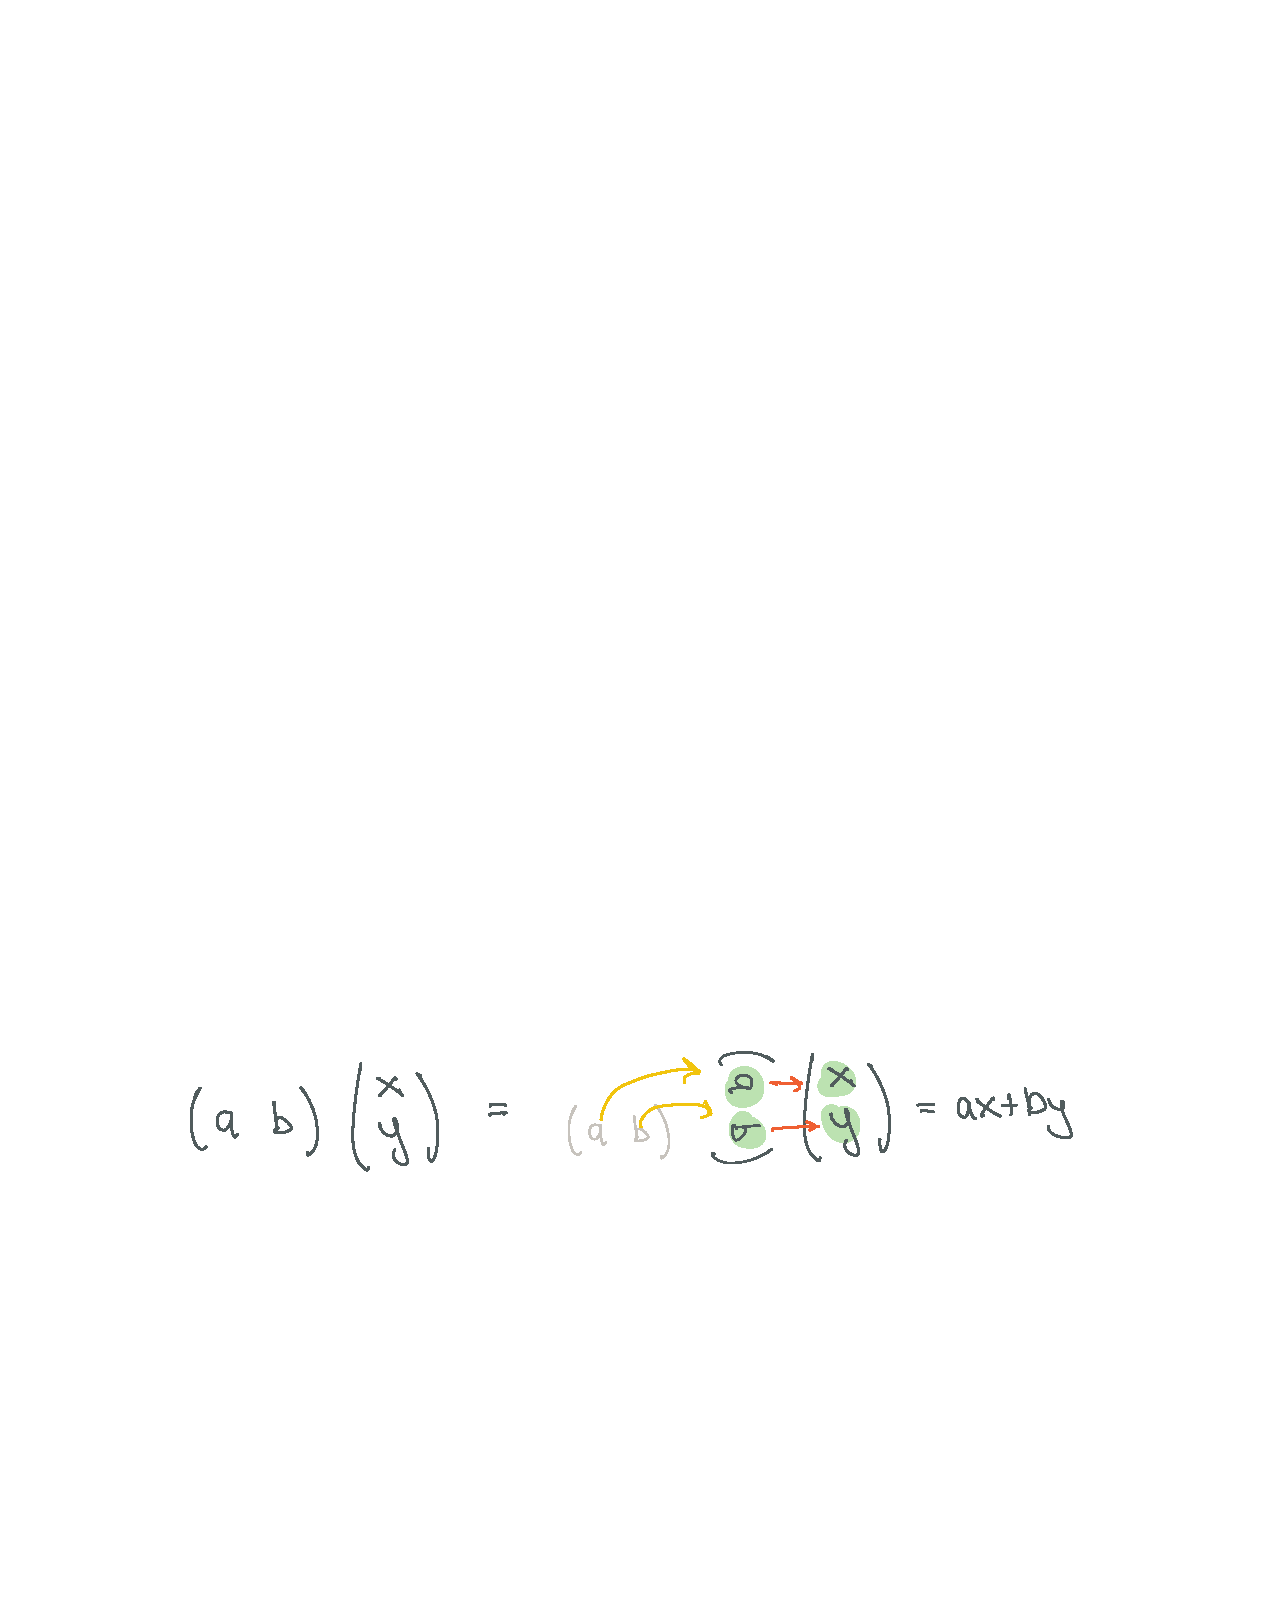
\includegraphics[width=.8\textwidth]{figures/MatrixMult_0220.pdf}
\end{figure}
Observe that the result of this multiplication is a number.
\begin{exercise}
Draw the vector
\begin{align}
    \vec{v} = \begin{pmatrix}
        1 \\ 1
    \end{pmatrix} \ .
\end{align}
Draw the vector
\begin{align}
    \begin{pmatrix}
        2 & 1 \\
        1 & 1
    \end{pmatrix}
    \begin{pmatrix}
        1 \\ 1
    \end{pmatrix} \ .
\end{align}
\end{exercise}

We can also multiply matrices with one another. The result of this is another matrix. One can construct the components of this matrix by thinking of the left matrix acting on each column of the right matrix to give the corresponding column of the matrix product. Here's how one would find the top-left component of the product of two $2\times 2$ matrices:
\begin{figure}[ht]
    \centering
    \captionsetup{font={scriptsize,sf}}
    \sidecaption[][-2\baselineskip]{%
        Multiplication of two matrices, highlighting the steps to find the top-left component of the product matrix.
        %
        %% \label command inside the \sidecaption command
        \label{fig:matrix:mult:2222a}
    }
    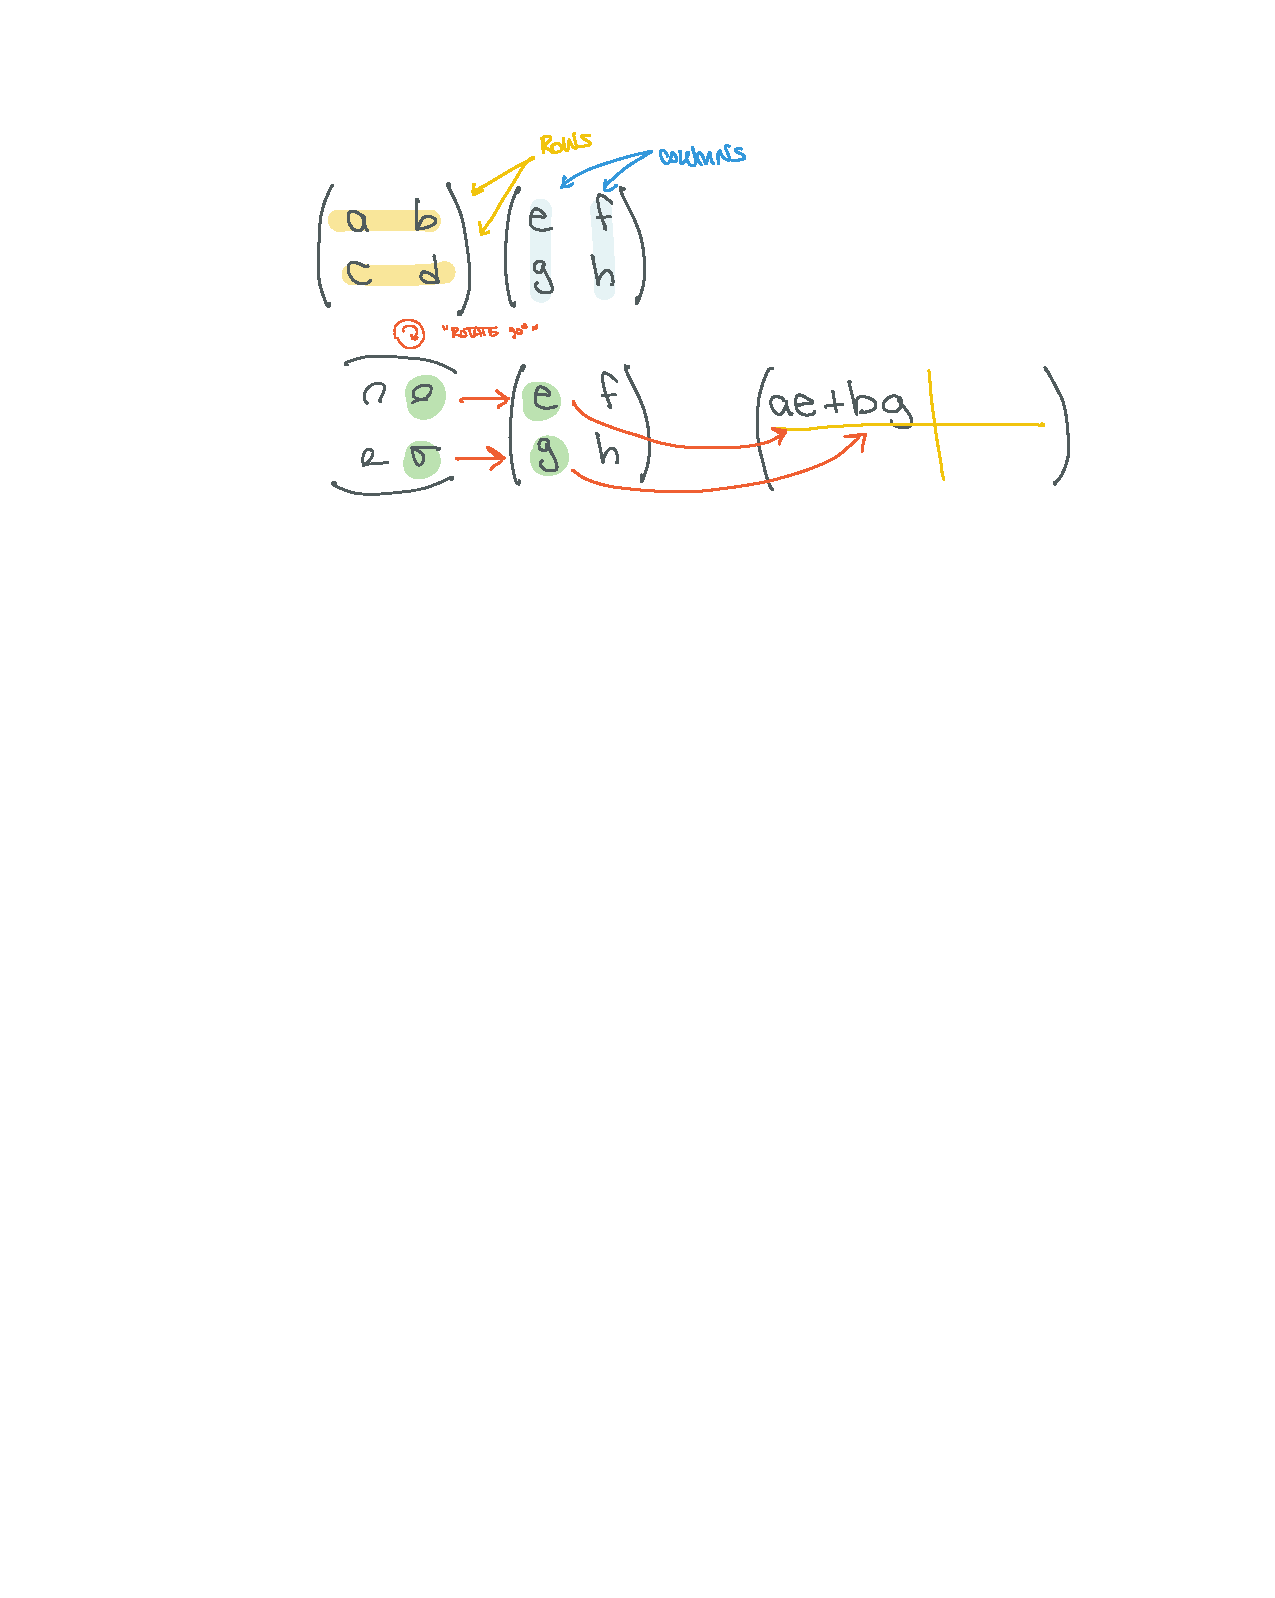
\includegraphics[width=.8\textwidth]{figures/MatrixMult_2222a.pdf}
\end{figure}
We can go on and find the top right (first row, second column) and bottom left (second row, first column) components of the product matrix, see Figure~\ref{fig:matrix:mult:2222b}.
\begin{figure}[ht]
    \centering
    \captionsetup{font={scriptsize,sf}}
    \sidecaption[][-2\baselineskip]{%
        Multiplication of two matrices, highlighting the steps to find the top right and bottom left components of the product matrix.
        %
        %% \label command inside the \sidecaption command
        \label{fig:matrix:mult:2222b}
    }
    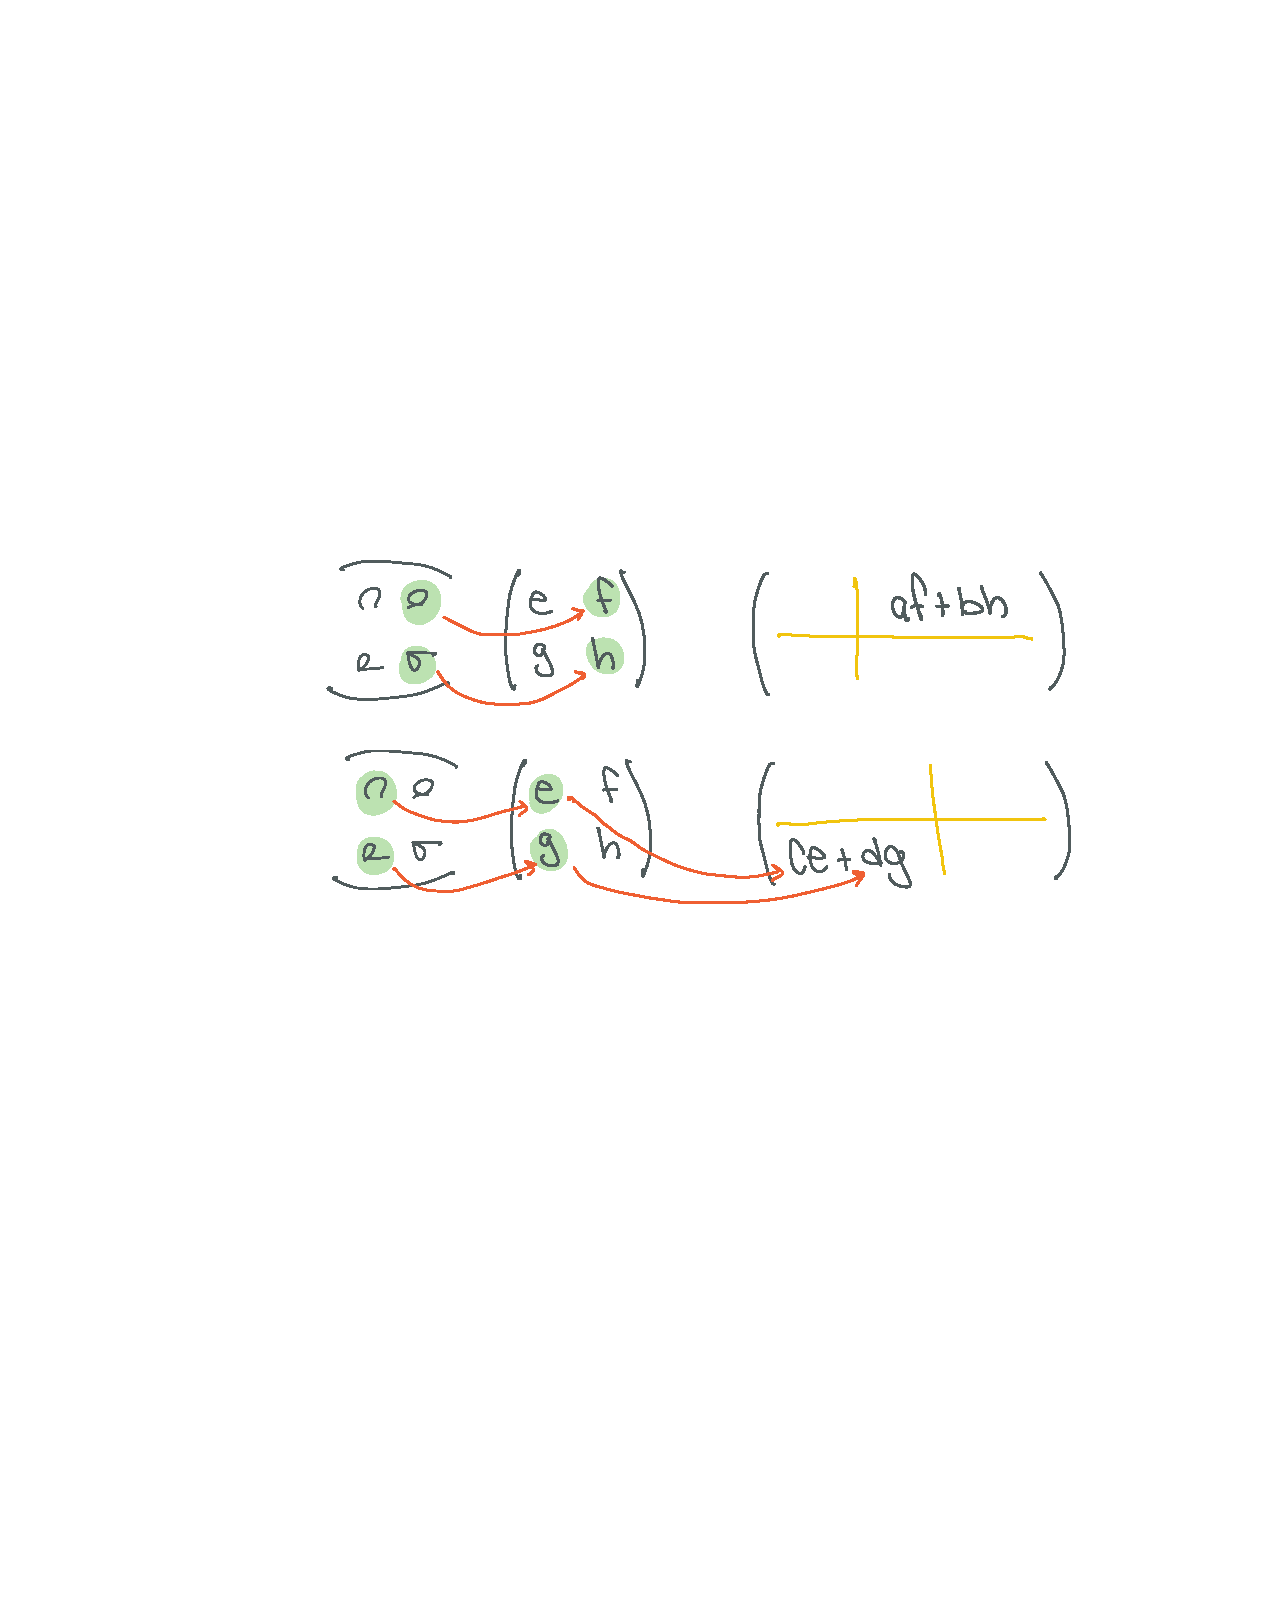
\includegraphics[width=.8\textwidth]{figures/MatrixMult_2222b.pdf}
\end{figure}
\begin{exercise}
Show that the product of two $2\times 2$ matrices $MN$ is different from the product in the opposite order, $NM$. We say that matrix multiplication is not commutative.  
\end{exercise}
\begin{exercise}
Show that
\begin{align}
\begin{pmatrix}
    2 & 1 \\
    1 & 1 
\end{pmatrix}
\begin{pmatrix}
    1 & -1 \\
    -1 & 2 
\end{pmatrix}
=
\begin{pmatrix}
    1 & 0 \\
    0 & 1
\end{pmatrix} \ .
\end{align}
The matrix on the right-hand side is called the \textbf{identity matrix}, $\one$, because when it acts on a vector it leaves the vector unchanged. We say that the two matrices on the left-hand side are \textbf{inverses}. Show further that if two matrices are inverses, $M$ and $M\inv$, then the order of the multiplication does not matter: $MM\inv M\inv M = \one$.
\end{exercise}

One can further generalize this to non-square matrices---that is, matrices with a different number of rows than columns. Those matrices will not be of direct use in this course. However, the rules of matrix multiplication follow.
\begin{exercise}
Show that you can use the matrix multiplication rules multiply a $2\times 3$ matrix onto a $3\times 2$ matrix, where our notation is $(\textnormal{number of rows})\times(\textnormal{number of columns})$.
\end{exercise}
\begin{exercise}
Show that you \emph{cannot} multiply a $2\times 3$ matrix onto a $2 \times 3$ matrix. 
\end{exercise}
\begin{exercise}
Suppose you want to multiply an $n\times m$ matrix onto a $k \times \ell$ matrix.. What are the conditions on the numbers $n, m, k, \ell$ for this to make sense using the matrix multiplication rule?
\end{exercise}



The rules for matrix multiplication also introduces the notion of a matrix inverse. Given a matrix $M$, the inverse of the matrix $M\inv$ `undoes' whatever the matrix does. It is also true that $M$ `undoes' whatever $M\inv$ does. In this sense $(M\inv)\inv = M$. The defining relation is
\begin{align}
    M M\inv = M\inv M = \one \ ,
    \label{eq:matrix:invers:multiplcation:notation}
\end{align}
where $\one$ is the identity matrix that is zero except for ones along the diagonal.\sidenote{When $\one$ acts on a vector it returns the same vector: $\one \vec{v} = \vec{v}$.}
\begin{exercise}\label{ex:matrix:inversino:the:hard:way}
Let us assign values to $M$ and $M\inv$ in the $2\times 2$ case:
\begin{align}
M &=
    \begin{pmatrix}
    a & b \\
    c & d    
    \end{pmatrix}
    &
M\inv &=
    \begin{pmatrix}
    x & y \\
    z & w    
    \end{pmatrix} \ .
\end{align}
Write out the \emph{four} conditions that we get from $MM\inv = \one$. \textsc{Partial answer}: one of the conditions is
\begin{align}
    ax + bz = 1 \ .
\end{align}
If you know each of the components of $M$, then you have four equations for four unknowns. This system of equations may have a solution.
\end{exercise}
\begin{exercise}
Using the system of equations above, prove the usual identity for $2\times 2$ invertible matrices:
\begin{align}
    M\inv = \frac{1}{ad-bc}
    \begin{pmatrix}
    \pp d & -b \\
    -c & \pp a    
    \end{pmatrix} \ .
\end{align}
\end{exercise}
All of this assumes that the inverse is well defined, which is not always the case. For example, if either a row or a column of $M$ is all zeros---the matrix will not be invertible. This is because the matrix \emph{projects out} information and there is no way to recover that information.



This notion of matrix multiplication is helpful and perhaps something you may have learned in earlier stages of your education. It is still the way I do many calculations. \emph{However}, the rules in this section are a \emph{shortcut} for a much richer mathematical structure. It is this mathematical structure that we want to reveal because it shows us how seemingly different mathematical structures in physics are actually rooted in the same underlying language. As such, many of the notions in this chapter may be ideas that you must first \emph{unlearn} in order to \emph{relearn} how they are outputs of the richer structure.\sidenote{When I teach this class there are often a few students who are apologetic for not having taken a formal linear algebra class. I have noticed that those students sometimes do much better in the course because they have fewer preconceptions to unlearn.}


\section{Rotations}\label{sec:Euclidean:three:space:rotations}

Rotations are transformations that take vectors into other vectors. They are a specific example of what is more generally known as an \emph{isometry}---and idea that we shall refer to over and over in this course. Your intuition about rotations may align with the following observations:
\begin{itemize}
    \item Rotations preserve the magnitude of vectors.
    \item Rotations preserve the angle between vectors. 
\end{itemize}
Because both magnitude and angle are related to the dot product, you may guess that rotations have something to do with the dot product. This is correct---but we need to build up some mathematical structure before we can articulate this idea carefully. In this section, we simply whet your appetite by saying that a `working definition' of rotations in Euclidean space of any dimension is that a rotation is a matrix $R$ that satisfies
\begin{align}
    R^\trans R = \one \ ,
    \label{eq:RTR:one}
\end{align}
where the \textbf{transpose} of a matrix $R^\trans$ is what happens when you flip all the elements along the diagonal:
\begin{align}
    \begin{pmatrix}
        a & b \\
        c & d
    \end{pmatrix}^\trans \defeq
    \begin{pmatrix}
        a & c \\
        b & d
    \end{pmatrix} \ .
\end{align}
We write $\one$ to mean the unit matrix: the matrix with only ones along the diagonal. Matrices $R$ that satisfy \eqref{eq:RTR:one} are called \textbf{orthogonal}\index{orthogonal}---this is just a fancy name for rotation. 

\begin{exercise}
Show that the standard form of a rotation in two dimensions,
\begin{align}
R=
    \begin{pmatrix}
    \cos \theta & -\sin\theta \\
    \sin \theta & \pp\cos\theta      
    \end{pmatrix} \ .
    \label{eq:2D:rotation:standard}
\end{align}
satisfies \eqref{eq:RTR:one}. Using this form of rotations, show that rotations in 2-dimensional Euclidean space preserve the length of vectors and the angle between vectors. \textsc{Hint}: use $\cos^2\theta + \sin^2\theta = 1$.
\end{exercise}

\begin{subappendices}
\section{Transpose}\label{sec:transpose}
The \textbf{transpose} of a matrix is what happens when you \emph{flip all the elements along the diagonal}.\sidenote{By \emph{diagonal} we mean the elements from the top left of the matrix down to the bottom right.} Given a matrix $M$, the transpose of $M$ is $M^T$ with components
\begin{align}
    (M^\trans)\aij{i}{j} &= M\aij{j}{i} \ .
    \label{eq:transpose:components}
\end{align}
This working definition of a transpose is not \emph{quite} the most useful one---but it is the most clear to write out.

\begin{example}
The following two matrices are transposes of each other.
\begin{align}
    M &= 
    \begin{pmatrix}
        9 & -3 & 2 \\
        2 & \pp 5 & 7 \\
        1 & \pp 0 & 3
    \end{pmatrix}
    &
    M^\trans &= 
    \begin{pmatrix}
        \pp 9 & 2 & 1 \\
        -3 & 5 & 0 \\
        \pp 2 & 7 & 3
    \end{pmatrix}
    \ .
\end{align}
\end{example}

This unusual operation will turn out to be rather useful for us. I leave the following cryptic statement: while the transpose of a matrix is \emph{not} its inverse, but it does have a \emph{dual} relationship to the original matrix. Once we define a metric, we will be able to give a more rigorous definition for transpose. For now, let use take \eqref{eq:transpose:components} as the definition of something we can do to matrices. We tackle this properly when we define the adjoint in Section~\ref{sec:adjoint}.


\section{Trace}

The \textbf{trace} of a matrix $M$ is simply the sum of its diagonal components:
\begin{align}
    \Tr M = M\aij{i}{i} = M\aij{1}{1} + M\aij{2}{2} + \cdots \ .
\end{align}
It is not obviously meaningful from the perspective of $M$ being a linear transformation. However, it ends up being useful as as a mechanical procedure that one can do to matrices. The reason for this is something we will see soon: the trace of a matrix is unchanged under rotations. 

\section{Determinant}
\label{sec:determinants:easy}


Here's another seemingly strange operation that you can do on a matrix. The determinant of a $2\times 2$ matrix is defined to be
\begin{align}
    \det M \equiv M\aij11 M\aij12 - M\aij12 M\aij21 \ .
\end{align}
Weird, right? Determinants for higher-dimensional square matrices can be defined recursively by taking specific linear combinations of sub-matrices. There are silly rules for this. There are fancy words for the sub-matrices (minors) and the appropriate sign for summing together those determinants (cofactors). Look, it's a mess. You should be able to calculate the determinant of a general $2\times 2$ matrix because it's easy. In case of national crisis, you should be able to calculate the determinant of a general $3\times 3$ matrix after consulting a reference to double check the signs.\sidenote{That reference will not be these notes.} However, at this stage we will not make a big deal about determinants. I think engineering classes make a big deal about determinants because they can help with solving systems of linear equations using matrices---but \emph{that's not the kind of linear algebra we're doing in physics}.

\begin{example}\label{eg:determinant:of:diagonal}
The determinant of a diagonal matrix is simply the product of each of its diagonal elements. 
\end{example}

In Chapter~\ref{ch:determinant} we take time to define the determinant properly.\sidenote{We are skipping all pretense of taking the determinant anything bigger than a $2\times 2$ matrix by hand. There are computers for that. Instead, let us figure out how to use the determinant.} 

\section{Cross product}

The cross product is an incredibly strange operation. It takes two vectors and returns another vector. Not only that, the \emph{order of the input vectors} matters. $\vec{v}\times\vec{w} = -\vec{w}\times\vec{v}$. The length of the cross product of two vectors is somehow related to the area of the parallelogram formed out of the two vectors. You have seen the cross product in your introductory physics courses: it shows up in the definition of angular momentum, the force law for a magnetic field, and the expression for the magnetic field from a vector potential. You would think that the cross product is a big part of our story. 

It is not.

The reason is that the cross product only exists in three dimensions. There is a structure that generalizes the cross product, but we first need to build up the mathematical machinery to use it. 

\section{The odd history of the vector}

I have find the history of mathematics strangely alien. As practicing physicists, we learn to \emph{use} mathematical ideas. Those who are formally inclined may lean into how these ideas are defined and generalized. But the question of ``how was it that humans came to define these ideas'' is rarely something we talk about.\sidenote{In contrast, there are plenty of great recollections of the \emph{need} to invent quantum mechanics or relativity. What was the \emph{need} to invent a vector? As American physics Nobel laureate Steven Weinberg would advise young colleagues, it is always worth it to learn the history of one's discipline.}

It should not be surprising that the history of vectors is intimately tied to physics. It may be a little more surprising that this history is also intimately connected to the history of calculus---here we wave our hands at the usual hagiographic stories of Newton and Leibniz that we like to tell in our field. I found this a \emph{little} surprising because I always thought of calculus as ``more sophisticated'' (and hence developed more recently) than vectors. What I found most surprising is that the concept of a vector is closely tied to complex analysis---a field that we do not often associate with vectorial objects---and at least one that I used to think was ``more sophisticated'' than calculus. We can point to the connection using Euler's identity:
\begin{align}
    \E^{\I\theta}  = \cos\theta + \I \sin\theta \ .
\end{align}
When we draw this, we represent $\E^{\I \theta}$ as a unit length arrow on the Cartesian plane. We say that $\cos\theta$ is the component along the $\hat x$-axis and $\sin\theta$ is the component along the $\hat y$-axis. We have drawn a two-dimensional vector. The arithmetic of complex numbers then maps onto the arithmetic of vectors. In my education, I was taught that ``of course'' this is how complex numbers and vectors work---what else would they do?

The history goes deeper. You may notice that complex numbers are different from vectors because we have a rule for multiplying complex numbers, but we do not have a rule for multiplying two-component vectors.\sidenote{``What about the cross product?'' There is no cross product for two-component vectors. There is a time to talk about the cross product---but for a large portion of this course, we do \emph{not} talk about the cross product.} If we look more carefully at the multiplication of complex numbers, we recognize that something about complex multiplication encodes rotation in the two dimensional plane. Specifically:
\begin{align}
    \E^{I\theta} \E^{I\varphi} = \E^{I(\theta+\varphi)} 
    = \cos(\theta+\varphi) + \I \sin(\theta+\varphi) \ .
\end{align}
In a more sophisticated language, we say that $\I$ \emph{generates} rotations in two dimensions. For a good portion of the 1800s, physicists sought a mathematical language to describe rotations in three dimensions. This is what William Rowan Hamilton\sidenote{Namesake of the Hamiltonian $\hat H$ and Hamiltonian mechanics, but otherwise unrelated to Alexander Hamilton of American history... \href{https://youtu.be/SZXHoWwBcDc}{youtu.be/SZXHoWwBcDc}} had been grappling with when he developed the theory of \textbf{quaternions}\index{quaternions}: an extension of complex numbers that included \emph{three} complex directions $i$, $j$, and $k$. These had the property that $i^2 = j^2 = k^2 = ijk = -1$. Unlike the relation of $\I$ to real numbers, the three distinct complex directions satisfy \emph{anticommutation} relations: $ij = -ji$. There is a moment when attentive physics students learn about quaternions and realize that they behave just like the generators of rotations acting on the spin-1/2 representation.\sidenote{Forgive me for jumping off into jargon here. As Gen-Z'ers say, \emph{if you know, you know}---but if you do not know, then the details are immaterial in this section.} All this is to say that one realizes that if Hamilton's $i$, $j$, and $k$ are actually the \textbf{Pauli matrices}\index{Pauli matrices} and if multiplication between Pauli matrices is mapped onto the commutator of those matrices, then one precisely realizes the properties of quaternions. The surprise here is that a generalization of complex numbers should have something to do with the simplest quantum mechanical system: the rotations of a spin-1/2 particle. My point here is that historically one should \emph{not} be so surprised. Ordinary complex numbers already encoded a \emph{representation}\sidenote{The word `representation' is also mathematical jargon, but we may take the colloquial meaning. A poetic definition is that a representation of an idea is related to the idea the same way shadows are related to people in Plato's allegory of the cave.} of rotations in two dimensions. This historical observation is central to the mathematical treatment of general symmetries, called \textbf{group theory}\index{group theory} and---more specifically---\textbf{representation theory}.\sidenote{The specific brand of representation theory is the representation of continuous groups, or the representation of so-called Lie algebras.}

William Rowen Hamilton imagined quaternions as a framework to describe how objects transform in three dimensions. He sought a mathematical framework to represent physical quantities that had magnitude and direction, where the direction can be acted upon by rotations. His realization that quaternions offer such a framework led him to famously scratch the quaternionic algebra into the Broom Bridge. This is the reason why some treatments of algebra---often in engineering courses for reasons I do not understand---use $i$, $j$, and $k$ to indicate the $\hat x$, $\hat y$, and $\hat z$ directions. These days, we do not talk about $i$, $j$, and $k$ as quaternions---Hamilton's invention largely comes off as a roadside curiosity on the highway of one's physics education. There is, however, more to this curiosity. The anticommutation relations of quaternions give a geometric interpretation to vector multiplication related to finding areas, volumes, and hyper-volumes formed by (hyper-)parallelograms\sidenote{A hyper-parallelogram is a parallelogram in more than two dimensions. The mathematical name for this is a parellelpiped.} of vectors. This is called \textbf{geometric algebra}\footnote{For an excellent summary in 30 minutes: \url{https://youtu.be/1cRFfYQYGxE}} and has recently had a quiet resurgence in mathematical physics. There is a reasonable argument for systematically incorporating geometric algebra into the physics curriculum~\autocite{Doran:2007tqa}\footnote{There is also room for lively counter-arguments: \url{https://alexkritchevsky.com/2024/02/28/geometric-algebra.html}}. The mathematically inclined may want to explore these topics further,\autocite{chisolm2012geometricalgebra,chappell2016geometricalgebranaturalrepresentation,brechet2022rotationsclassicalmechanicsusing,lundholm2009cliffordalgebrageometricalgebra,brechet2022electrodynamicsgeometricalgebra,Lasenby:2019gmi,almeida2005geometricalgebraparticledynamics} where applications even span contemporary applications in machine learning and robotics.\autocite{hitzer2013introductioncliffordsgeometricalgebra} For more on the history of the concept of vectors, I highly recommend \emph{Vector} by Robyn Arianrhod, see Fig.~\ref{fig:arianrhod}.
\begin{marginfigure}%[th]
    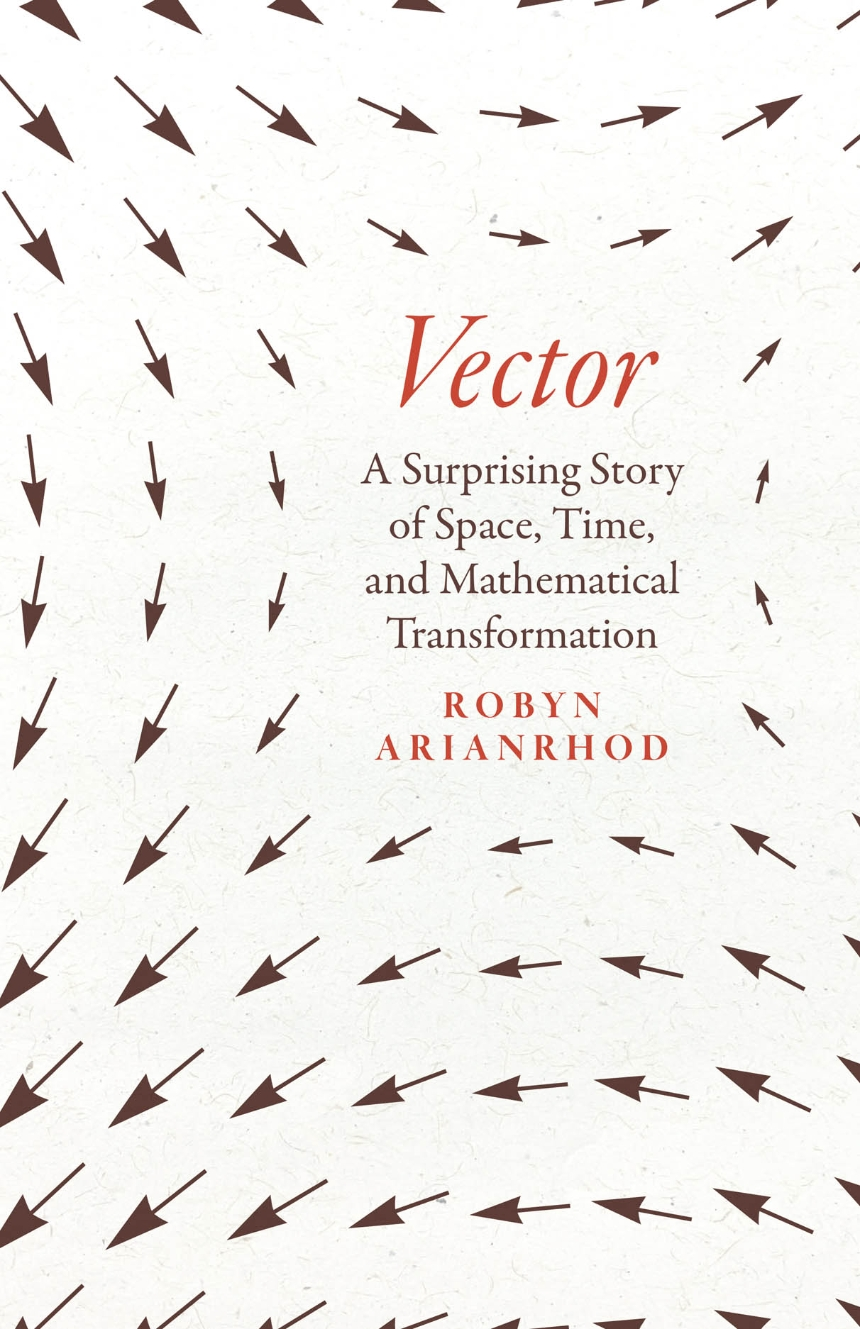
\includegraphics[width=.8\textwidth]{figures/VectorArianrhod.jpg}
    \captionsetup{font={scriptsize,sf}}
    \caption{\cite{arianrhod2024vector}}
    \label{fig:arianrhod}
\end{marginfigure}


% \autocite{ogawa2009housekeeper}

\end{subappendices}
